% Working report based on the supplied DA241O final term paper template.
% Overleaf main document: main.tex. Compile with pdfLaTeX.
% Unfinished sections retain the template's instructional placeholders.
% The explicit page breaks before References and the back matter reproduce
% the supplied template; remove/adapt those breaks when writing the report.
\documentclass[12pt,a4paper]{article}
\usepackage[T1]{fontenc}
% Latin Modern follows the Computer Modern typography of Assignments 1 and 2.
\usepackage{lmodern}
\usepackage{microtype}
\usepackage{graphicx}
\usepackage[section]{placeins}
\usepackage{caption}
\captionsetup[figure]{font=small,labelfont=bf,justification=raggedright,singlelinecheck=false,skip=7pt}
\usepackage[margin=1in]{geometry}
\usepackage{setspace}
\onehalfspacing
\setlength{\parindent}{0pt}
\setlength{\parskip}{6pt}
\usepackage{titlesec}
\titleformat{\section}{\large\bfseries}{\thesection.}{0.6em}{}
\titleformat{\subsection}{\normalsize\bfseries}{\thesubsection}{0.6em}{}
\titlespacing*{\section}{0pt}{1.2em}{0.45em}
\titlespacing*{\subsection}{0pt}{0.85em}{0.3em}
\usepackage{fancyhdr}
\pagestyle{fancy}
\fancyhf{}
\fancyhead[L]{DA241O: Managerial Economics}
\fancyhead[R]{Final Term Paper}
\fancyfoot[C]{\thepage}
\renewcommand{\headrulewidth}{0.4pt}
\setlength{\headheight}{14.5pt}
\addtolength{\headsep}{-2.5pt}
\usepackage[hidelinks]{hyperref}
\usepackage{tabularx}
\captionsetup[table]{font=small,labelfont=bf,justification=raggedright,singlelinecheck=false,skip=5pt}
% O3 additions: macros used in the O3 text
\providecommand{\HHI}{HHI}
\providecommand{\CRtwo}{CR2}

% The source prints its bullets as ordinary, unindented paragraphs.
\newcommand{\templatebullet}[1]{\par\noindent\textbullet\hspace{5.88pt}#1\par}

\begin{document}
\hypersetup{pageanchor=false}
\begin{titlepage}
\centering
\vspace*{2cm}
{\Large\bfseries DA241O: MANAGERIAL ECONOMICS\par}
\vspace{1.5cm}
{\LARGE\bfseries Final Term Paper\par}
\vspace{1.5cm}
{\Large\bfseries [Title of the Study]\par}
\vspace{2cm}
{\large\textbf{Team Name:} [Team Name]\par}
\vspace{0.75cm}
{\large\textbf{Team Members:}\par}
\vspace{0.3cm}
{\large Name 1\\
Name 2\\
Name 3\\
Name 4\par}
\vfill
{\large DA241O: Managerial Economics\\
Department / Programme\\
Date of Submission\par}
\end{titlepage}
\hypersetup{pageanchor=true}
\setcounter{page}{1}

\section*{Abstract}
Briefly present the research problem, research question, data and methodology, main findings, and key implications.

\vspace{0.5cm}
\textbf{Keywords:} [Keyword 1]; [Keyword 2]; [Keyword 3]; [Keyword 4]

\section{Introduction}
\subsection{Background and Problem Statement}
Introduce the market, firm, sector, or policy setting being studied and explain the problem being investigated.

% ===== O3 START (1.1) =====
\textbf{O3 (entrant airlines).} Between 2015 and 2026, nine new airlines began scheduled domestic service in India: Vistara, Akasa Air, TruJet, Star Air, Fly91, Flybig, Zoom Air, India One Air and Air Deccan. O3 asks what became of the entrants: did any become a meaningful and lasting competitor, or did the entries leave the market structure unchanged?
% ===== O3 END =====

\subsection{Research Question}
State the primary research question.

\subsection{Research Objectives}
State the 2--3 research objectives.

% ===== O3 START (1.3) =====
\textbf{O3.} Track the nine entrants over time and assess whether they became meaningful and persistent competitors, using passenger share, route presence and financial and funding evidence.
% ===== O3 END =====

\subsection{Economic Framework}
Identify the economic concept or framework used in the study and explain its relevance to the research question.

Examples may include demand and supply, market structure, information asymmetry, adverse selection, network effects, opportunity cost, principal-agent problems, or other relevant concepts from the course.

% ===== O3 START (1.4) =====
\textbf{O3.} O3 uses economies of scale (average cost AC = F/Q + v, so more output spreads fixed cost over more passengers) and break-even reasoning to ask why some entrants persist while others exit.
% ===== O3 END =====

\subsection{Scope of the Study}
Specify the relevant market, geography, time period, population, firms, products, or other boundaries of the study.

% ===== O3 START (1.5) =====
\textbf{O3.} The nine entrants (Vistara, Akasa Air, TruJet, Star Air, Fly91, Flybig, Zoom Air, India One Air and Air Deccan); scheduled domestic passenger service; January 2015 to July 2026; national passenger shares for all nine; route evidence for Vistara, Akasa Air and TruJet; audited financial results for Vistara and Akasa Air only, with funding evidence for all three case-study airlines.
% ===== O3 END =====

\section{Literature Review}
\subsection{Existing Literature}
Review the relevant academic, government, industry, and other credible sources.

% ===== O3 START (2.1) =====
\textbf{O3.} Oliveira and Oliveira (2018) show that effective competition on city pairs depends on more than the number of carriers present. Wang et al. (2018) link low-cost competition in India to lower fares and higher air travel demand. Grosche et al. (2020) find concentration rising after a large carrier's bankruptcy, and case studies trace the failures of Jet Airways (Soman \& Punjani, 2024) and Go First (Jasrotia et al., 2025) to financial distress. Jayathilakan et al. (2024) find Indian airline revenue positively associated with passenger volume, and Kumari et al. (2026) study market behaviour in Indian aviation at the brand level.
% ===== O3 END =====

\subsection{Synthesis of Literature}
Discuss the major findings, patterns, and differences across the literature.

% ===== O3 START (2.2) =====
\textbf{O3.} The studies suggest that low-cost competition expands demand while concentration rises when a large carrier fails, but they treat new entrants as part of aggregate market structure rather than as a group followed over time.
% ===== O3 END =====

\subsection{Research Gap}
Clearly identify what is not adequately addressed by the existing literature and how the present study addresses this gap.

% ===== O3 START (2.3) =====
\textbf{O3.} Among the sources reviewed for this study, none follows a cohort of new entrants by age and combines national share, route presence and financial evidence. O3 does this for the nine entrants.
% ===== O3 END =====

\subsection{Relevance to the Present Study}
Explain how the existing literature and identified gap inform the research question and analysis.

% ===== O3 START (2.4) =====
\textbf{O3.} The gap motivates tracking each entrant from its first month, and the entrants' combined share supplies the fringe against which O4's duopoly cut-offs are read.
% ===== O3 END =====

\section{Data and Methodology}
\subsection{Research Design}
Briefly describe the research design used in the study.

% ===== O3 START (3.1) =====
\textbf{O3.} Descriptive and case-based design with three layers: national tracking of the nine entrants in event time, three case studies (Vistara, TruJet and Akasa Air, one per outcome), and financial and funding evidence.
% ===== O3 END =====

\subsection{Data Sources}
Describe the data source or sources, period covered, geographic coverage, sample or number of observations where applicable, and data collection procedure where applicable.

% ===== O3 START (3.2) =====
\textbf{O3.} National passenger shares come from DGCA monthly airline statistics as cleaned by Kubicek (2026): 1,577 scheduled domestic airline-months, January 2015 to July 2026 (April 2020 missing). Route shares use DGCA approved domestic schedules: 20 major routes (April 2019 to July 2026) and 30 airport pairs from TruJet's own filings (April 2019 to February 2020 and November 2021 to January 2022). Financials come from ICRA's audited tables for Tata SIA Airlines (Vistara) and SNV Aviation (Akasa Air) (ICRA, 2024; ICRA, 2026). Funding and outcome evidence comes from company releases, filings and press reports (Appendix B).
% ===== O3 END =====

\subsection{Unit of Analysis}
Clearly identify the unit of analysis, such as firm, product, transaction, household, district, city, industry, or another relevant unit.

% ===== O3 START (3.3) =====
\textbf{O3.} The airline brand as named by DGCA, observed by month; for route evidence, the airport pair (both directions pooled).
% ===== O3 END =====

\subsection{Variables and Measures}
Define the key variables, indicators, measures, or categories used in the analysis.

For quantitative studies, identify the dependent variable, main explanatory variables, and relevant control variables where applicable.

% ===== O3 START (3.4) =====
\textbf{O3.} Passenger share, event time $\tau$, scheduled-frequency share, route brand \HHI{}, net margin, revenue growth and load factor, plus the meaningful and persistent flags; see Appendix A.
% ===== O3 END =====

\subsection{Method of Analysis}
Explain the analytical method used and why it is appropriate for the research question and data.

Examples may include:
\templatebullet{Descriptive analysis}
\templatebullet{Comparative analysis}
\templatebullet{Regression analysis}
\templatebullet{Market concentration measures}
\templatebullet{Price analysis}
\templatebullet{Index construction}
\templatebullet{Cost-benefit analysis}
\templatebullet{Cost-effectiveness analysis}
\templatebullet{Case analysis}
\templatebullet{Qualitative analysis}

% ===== O3 START (3.5) =====

\textbf{O3.} Event-time tracking: months are renumbered from $\tau=0$ at the first month with passengers, and each entrant's share is recorded at $\tau=12,24,36$, with peak share, months active and outcome. An entrant is \emph{meaningful} if its share reaches 1\% in at least one month and \emph{persistent} if it stays at or above 1\% for 24 consecutive months; both cut-offs are study-defined. Airlines still flying are right-censored at July 2026. An airline's scheduled-frequency share on an airport pair is $100\times$ its scheduled flights divided by all recorded scheduled flights that month, and route brand \HHI{} is the sum of squared shares. Event time compares airlines at the same stage; route and financial evidence are added because national share understates a regional airline's local role and does not show whether growth was sustainable. Claims are limited to market structure, not fares or market power.
% ===== O3 END =====

\subsection{Hypotheses or Expected Relationships}
State the hypotheses or expected relationships developed during the research process, where applicable.

% ===== O3 START (3.6) =====
\textbf{O3.} \textbf{H7:} most entrants stay below 1\% of passengers or exit. \textbf{H8:} TruJet supplied at least half of scheduled flights on a majority of the airport pairs in its filings. \textbf{H9:} revenue growth is accompanied by an improving net margin.
% ===== O3 END =====

% Keep the first O4 description and figure together in this working draft.
\clearpage
\section{Descriptive and Exploratory Analysis}
\subsection{O4: National concentration trends}
Figure~\ref{fig:o4-national-eda} summarises 138 observed months from January 2015 to July 2026. The two largest ownership groups' combined passenger share (CR2) rises from 60.7\% to 91.3\%, while their share gap increases from 12.5 to 43.4 percentage points. The leading pair is IndiGo and Jet Airways Group in January 2015, and IndiGo and Air India Group in July 2026; groups are ranked afresh each month.

The January 2022 movement includes the study's inclusion of Vistara and AirAsia India/AIX Connect in the Air India Group. It should therefore not be attributed entirely to changes in airline passenger volumes. April 2020 is missing and is not interpolated.

\begin{figure}[htbp]
\centering
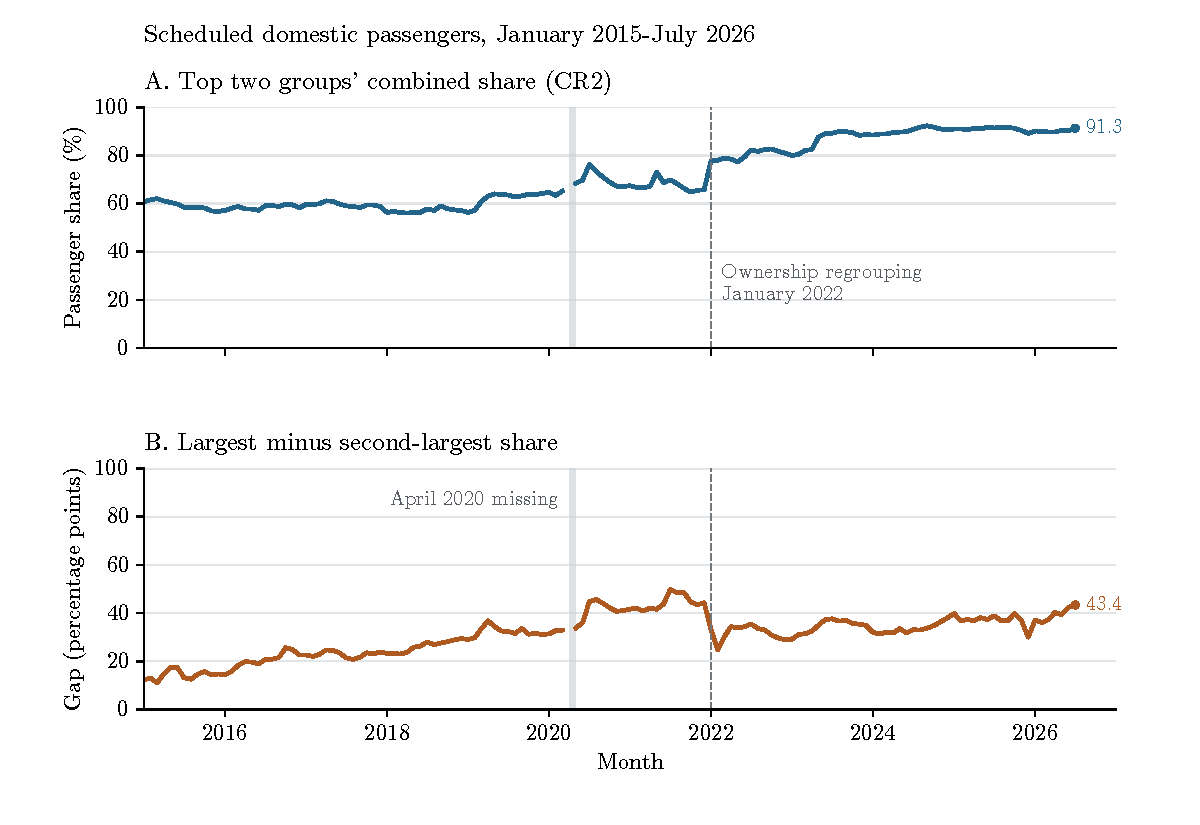
\includegraphics[width=\linewidth]{figures/o4_national_cr2_share_gap.pdf}
\caption{National concentration and share asymmetry, 2015--2026.}
\label{fig:o4-national-eda}
\vspace{2pt}
\begin{minipage}{\linewidth}
\footnotesize\setstretch{1.1}
\textit{Source:} DGCA monthly traffic via \href{https://github.com/mkubicek/india-aviation-stats/tree/16770ac59dae61ce7b80fd8bd67dd7f4cef280a6}{Kubicek (2026)}; authors' calculations.
\end{minipage}
\end{figure}


% ===== O3 START (4) =====
\subsection{O3: Entrant passenger shares by age}
\footnotesize\textit{Source note: national shares use the same cleaned DGCA file as the O4 analysis (Kubicek, 2026); the O3 figures are identical on commit \texttt{16770ac} (Assignment~2) and commit \texttt{bce8fc7} (1,577 scheduled domestic airline-months to July 2026). Route shares use the DGCA approved domestic schedules; financial inputs are from ICRA's audited tables (ICRA, 2024; ICRA, 2026). The route and financial calculations and their checks are in the team's O3 case-study repository.}\normalsize



Table~\ref{tab:o3-summary} summarises the nine entrants. Only Vistara and Akasa Air ever exceeded 1\% of domestic passengers. Together they carried 93\% of all passengers flown by the nine, and the other seven together never exceeded 1.2\% of passengers in any month (maximum 1.17\%, July 2026). All four entrants that ceased flying (TruJet, Flybig, Zoom Air, Air Deccan) were regional carriers whose peak share was below 0.8\%. Figure~\ref{fig:o3-life} in Appendix B shows each airline's operating span.

\begin{minipage}{\textwidth}
\footnotesize
\setlength{\tabcolsep}{3pt}
\captionof{table}{O3: Passenger share at $\tau=12,24,36$, peak share and outcome of the nine entrants}
\label{tab:o3-summary}
\noindent\begin{tabularx}{\textwidth}{|X|l|l|r|r|r|r|r|l|}
\hline
\textbf{Airline} & \textbf{First} & \textbf{Last} & \textbf{Months} & \textbf{$\tau{=}12$} & \textbf{$\tau{=}24$} & \textbf{$\tau{=}36$} & \textbf{Peak} & \textbf{Outcome} \\
\hline
Vistara & Jan 2015 & Nov 2024 & 118 & 1.97 & 3.27 & 3.58 & 10.44 & Merged \\
\hline
Akasa Air & Aug 2022 & Jul 2026 & 48 & 4.24 & 4.51 & 5.43 & 6.36 & Operating \\
\hline
TruJet & Jul 2015 & Feb 2022 & 79 & 0.35 & 0.48 & 0.44 & 0.76 & Ceased \\
\hline
Star Air & Jan 2019 & Jul 2026 & 90 & 0.09 & 0.20 & 0.23 & 0.73 & Operating \\
\hline
Fly91 & Mar 2024 & Jul 2026 & 29 & 0.08 & 0.23 & -- & 0.47 & Operating \\
\hline
Flybig & Jan 2021 & Oct 2025 & 58 & 0.11 & 0.17 & 0.00 & 0.24 & Ceased \\
\hline
Zoom Air & Feb 2017 & Jun 2018 & 16 & 0.03 & -- & -- & 0.04 & Ceased \\
\hline
India One Air & Oct 2022 & Jul 2026 & 46 & 0.01 & 0.02 & 0.02 & 0.02 & Operating \\
\hline
Air Deccan & Dec 2017 & Mar 2020 & 13 & -- & -- & -- & 0.01 & Ceased \\
\hline
\end{tabularx}
\par\footnotesize Shares are percent of all scheduled domestic passengers in the month; $\tau$ is calendar months since the first month with passengers; ``--'' means the airline had stopped, or had not yet reached that age, by July 2026. Operating airlines are observed only to July 2026. Source: DGCA via Kubicek (2026); authors' calculations.
\end{minipage}\par\medskip


\textbf{Result 1: scale entrants grow fast and persist; regional entrants do not.} Akasa Air reached 1\% of passengers in its third month and 3\% in its eighth, with 4.24\%, 4.51\% and 5.43\% at $\tau=12,24,36$. Vistara reached 1\% in its fourth month but had 1.97\%, 3.27\% and 3.58\% at the same ages, so at three years Akasa carried about 1.5 times its share (Figure~\ref{fig:o3-age}). Vistara stayed at or above 1\% in 115 of its 118 months and Akasa in 46 of 48, so both are persistent; the other seven fail the test. Over whole operating years, Vistara's share rose from 1.32\% to 3.61\% (year one to year three), Akasa's from 2.97\% to 4.84\% and TruJet's from 0.35\% to 0.39\%. In July 2026 the market carried about 12.0 million passengers, so Akasa's 5.54\% is about 665,000 passengers a month and one percentage point of share is about 120,000.

\begin{figure}[htbp]
\centering
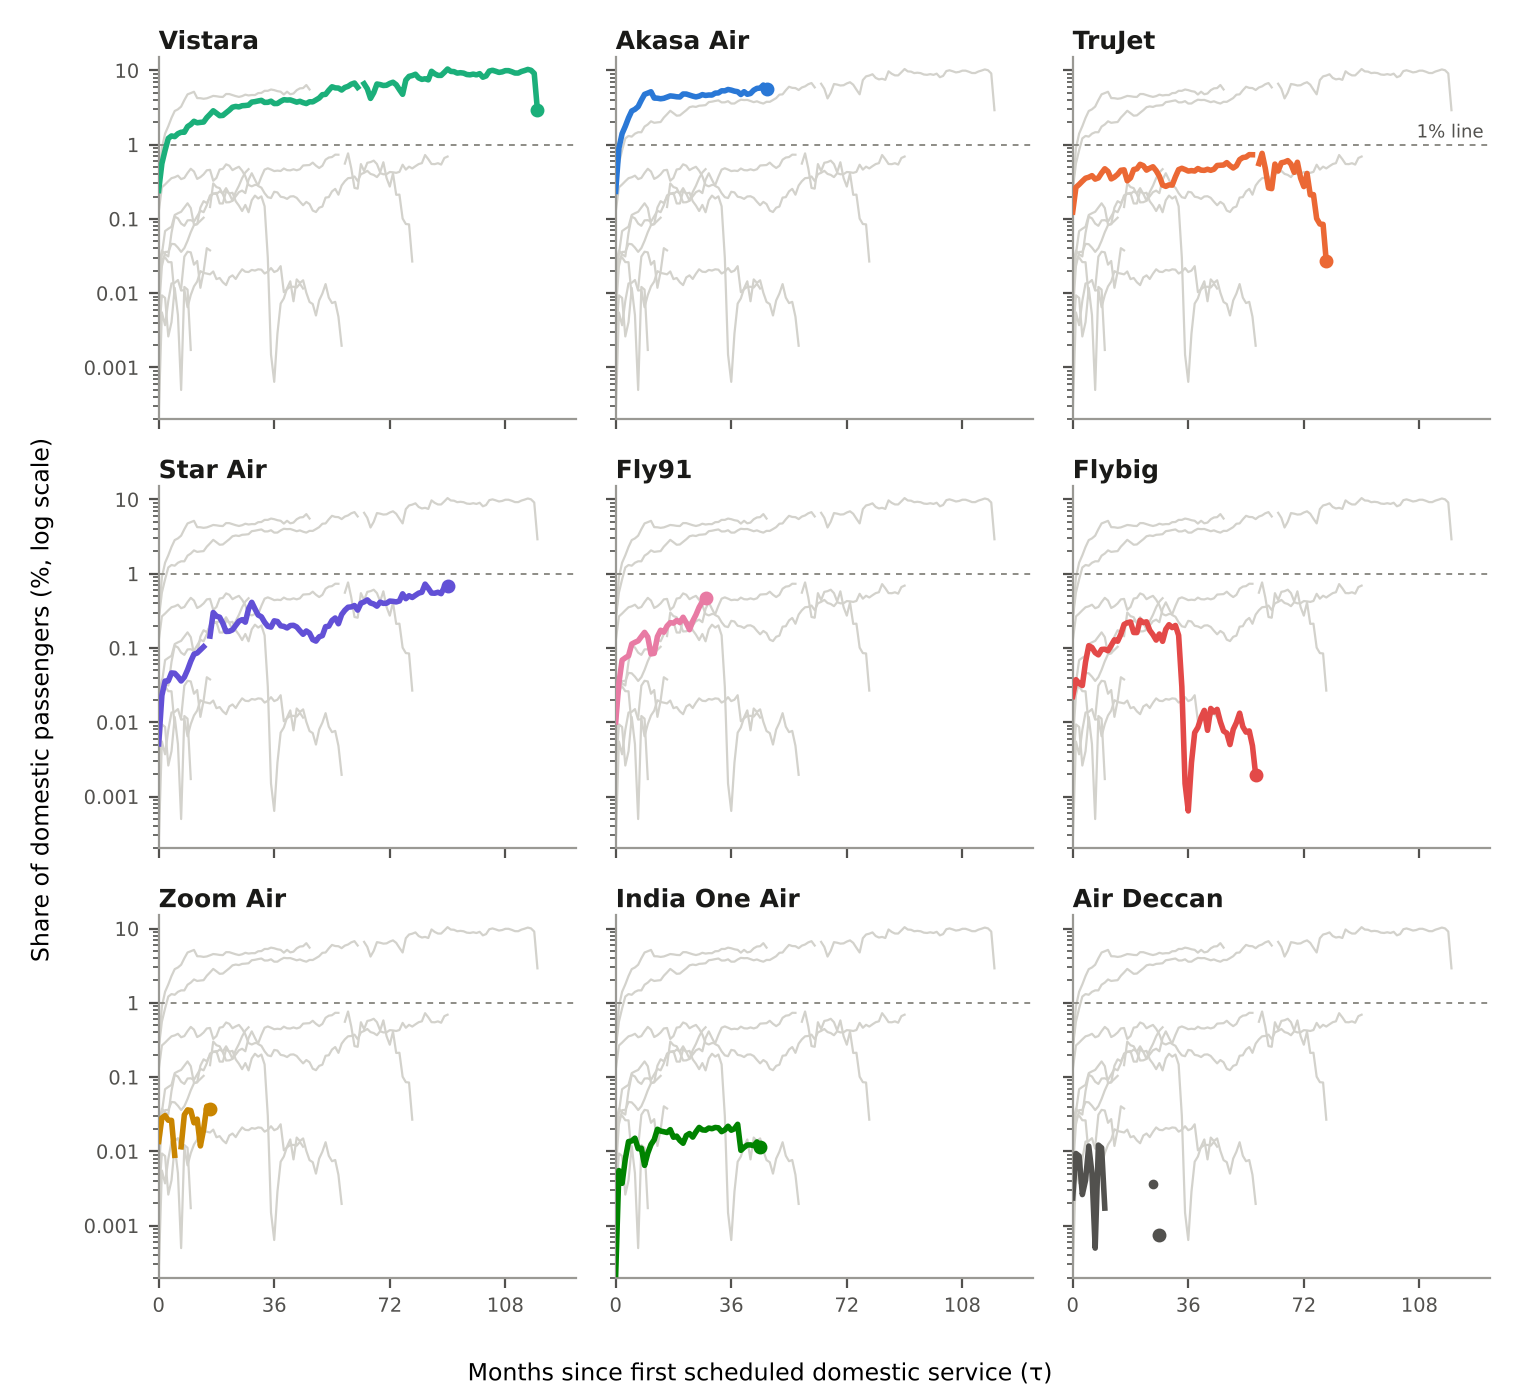
\includegraphics[width=0.92\textwidth]{figures/fig_o3_age.png}
\caption{O3: Passenger share of the nine entrants by months since first service (log scale). Vistara and Akasa Air are highlighted; the seven regional entrants are grey. Shares below 0.01\% are drawn at the axis floor; dots mark each airline's last observed month; Vistara's last point (November 2024) is a partial month. Source: DGCA via Kubicek (2026); authors' calculations.}
\label{fig:o3-age}
\end{figure}


% ===== O3 END =====

\section{Analysis and Results}
Present the main analysis and findings.

The specific form of analysis will depend on the research question and methodology. This section may include statistical results, regression results, calculated measures or indices, comparative results, tables and figures, qualitative findings, or other relevant empirical evidence.

Interpret the results in terms of their economic meaning and relevance to the research question.

% ===== O3 START (5) =====
\subsection{O3: Entrant outcomes, route presence and finances}
\textbf{Result 2: step gains coincide with rivals' exits.} Vistara averaged 3.88\% in the twelve months before Jet Airways stopped flying and 5.86\% in the eleven months after, a gain of about 2.0 points or roughly 235,000 passengers a month at the market's size then. Akasa averaged 2.43\% in the eight months before Go First stopped flying and 4.50\% in the twelve months after, a gain of about 2.1 points or roughly 270,000 passengers a month. These before--after differences also coincide with each airline's own fleet growth, so they show timing, not causation. They agree with Grosche et al.\ (2020), who find concentration rising after a large carrier's bankruptcy, and with case studies that link Jet Airways' decline to low-cost competition (Soman \& Punjani, 2024) and Go First's collapse to financial distress (Jasrotia et al., 2025).

\textbf{Result 3: local presence on routes.} National share understates TruJet's local role. In November 2019, 22 of the 30 airport pairs in its filing could be screened, and TruJet supplied at least half of the recorded scheduled flights on 17 of them (77.27\%); on 14 it was the only airline in the recovered schedules. Chennai--Salem had 60 TruJet flights out of 60 recorded (share 100\%, route \HHI{} 10,000), yet city-pair returns show only 3,281 passengers on that route across all airlines, and TruJet's national share was 0.63\%. On Mumbai--Delhi, Vistara's frequency share rose from 20.01\% (April 2019) to 31.27\% (February 2024) and Akasa's from 2.65\% (December 2022) to 8.75\% (July 2026). Between first and last covered month, Vistara's share rose on 16 of 20 routes but Akasa's on only 10 of 18, so Akasa's gains are uneven. These comparisons cover different periods and are not matched by airline age, and route brand \HHI{} counts Vistara and Air India as separate firms although both were Tata-owned by 2023.

\textbf{Result 4: financial performance and funding.} Table~\ref{tab:o3-fin} shows that revenue growth came with a much smaller loss for Vistara but not for Akasa. Akasa's FY2026 loss of Rs~2,716 crore is about Rs~3,150 per domestic passenger carried (8.6 million), an indicative figure because the loss also covers international flying. If each extra rupee of revenue contributed fully to profit, Akasa would need Rs~2,716 crore more revenue (44\% of its FY2026 base) to close its accounting loss, against Rs~581 crore (3.8\%) for Vistara; the contribution rate is an assumption. For TruJet, a 2021 report says an agreed investment had not arrived and its main investor had returned ownership to the founder, and by February 2022 reports describe groundings and one aircraft still flying (Hindu BusinessLine, 2021; ch-aviation, 2022). The UDAN audit records 52 route awards and 42 commencements for TruJet and none operational in March 2023 (Comptroller and Auditor General of India, 2023). ICRA records that equity and aircraft sale-and-leaseback inflows fund Akasa's continuing losses (ICRA, 2026), and Vistara's owners stated that merging it into Air India would join Air India's slots and traffic rights to Vistara's customers and capabilities (Singapore Airlines, 2022).

\begin{minipage}{\textwidth}
\footnotesize
\captionof{table}{O3: Financial results and funding of the three case-study airlines}
\label{tab:o3-fin}
\noindent\begin{tabularx}{\textwidth}{|>{\raggedright\arraybackslash}p{0.17\textwidth}|>{\raggedright\arraybackslash}X|>{\raggedright\arraybackslash}X|>{\raggedright\arraybackslash}X|}
\hline
 & \textbf{Vistara (FY2023$\to$FY2024)} & \textbf{Akasa Air (FY2025$\to$FY2026)} & \textbf{TruJet} \\
\hline
Operating income (Rs crore) & 12,261.4 $\to$ 15,310.3 & 4,582.7 $\to$ 6,167.9 & Not available \\
\hline
Profit after tax (Rs crore) & $-1{,}393.3\to-581.1$ & $-1{,}983.5\to-2{,}716.0$ & Not available \\
\hline
Net margin & $-11.36\%\to-3.80\%$ & $-43.28\%\to-44.03\%$ & -- \\
\hline
Year-3 load factor & 84.67\% & 91.01\% & 76.59\% \\
\hline
Funding & Rs~10,020 crore from Tata and Singapore Airlines by Aug 2024 & Equity round completed 19 Aug 2025; about US\$125 million is a press estimate & US\$25 million sought Feb 2022; receipt not verified \\
\hline
\end{tabularx}
\par\raggedright\footnotesize Vistara is standalone and Akasa consolidated; both include international services and give one annual change each, in different years. Sources: Akasa Air, 2025a; Business Standard, 2025; ICRA, 2024; ICRA, 2026; ch-aviation, 2022; authors' calculations.
\end{minipage}\par\medskip


% ===== O3 END =====

\section{Discussion}
Discuss the findings in relation to:
\templatebullet{The research question}
\templatebullet{The economic framework}
\templatebullet{The existing literature}
\templatebullet{The hypotheses or expected relationships}
\templatebullet{The broader context of the study}
Clearly state whether the hypotheses or expected relationships were supported, partially supported, or not supported, where applicable.

% ===== O3 START (6) =====
\subsection{O3: Entrant outcomes in light of the framework and literature}

Nine entrants in eleven and a half years produced two meaningful and persistent competitors, and one of them (Vistara) merged into Air India in November 2024. Akasa Air is the only entrant still growing as an independent rival at the cutoff, and it depends most on outside funding. Under $AC=F/Q+v$, entrants with more output spread fixed cost further: year-3 load factors were 84.7\% for Vistara (65.6\% in year one) and 91.0\% for Akasa (84.7\% in year one), against 76.6\% for TruJet, which fell from 80.1\% in year one. TruJet held most flights on its routes, but those routes were so small that a 100\% share meant a few thousand passengers a month, too little to cover aircraft and operating costs. Differentiation also differed: Vistara premium, Akasa low-cost, TruJet regional. Accounting profit excludes the opportunity cost of investors' capital, so funded losses at Akasa are not economic profit.

The result echoes Oliveira and Oliveira (2018): growth attracts entry, but effective competition needs more than the presence of carriers. Wang et al.\ (2018) link low-cost competition in India to lower fares and higher demand, which fits Akasa's fast growth as a low-cost carrier. Jayathilakan et al.\ (2024) find revenue positively associated with passenger volume, but here revenue growth alone did not secure survival or margin improvement. Brand-level measures (Kumari et al., 2026) count each entrant as a separate firm although seven of the nine carried a negligible share, and Vistara, a Tata-linked venture in which Singapore Airlines held 49\% (Tata Sons, 2024), is grouped with the Air India Group from January 2022 in O1.

For O4: in July 2026 IndiGo held 67.35\% of passengers and the Air India Group 23.96\%, so \CRtwo{} was 91.3\% and the fringe 8.7\%. Akasa's 5.54\% is about 64\% of that fringe, and all other airlines together hold about 3.2\%. The duopoly's resilience therefore depends on whether Akasa keeps growing, while regional entrants contribute little to it.


\subsection{O3: Hypotheses}

\textbf{H7 (most entrants stay below 1\% or exit): supported.} Seven of the nine entrants never reached 1\%, and five no longer operate independently (four ceased, one merged). The two that passed the 1\% test were both scale entrants.

\textbf{H8 (TruJet supplied at least half of scheduled flights on a majority of its screened airport pairs): supported for the sampled routes.} It did so on 17 of 22 screened pairs (77.27\%) in November 2019. The sample covers only recovered schedules.

\textbf{H9 (revenue growth is accompanied by an improving net margin): partially supported.} Vistara's net margin improved by 7.57 points with 24.87\% revenue growth; Akasa's worsened by 0.75 points with 34.59\% growth. Revenue growth alone did not ensure better margins.


% ===== O3 END =====

\section{Implications and Recommendations}
Discuss the implications of the findings for the relevant stakeholders.

Depending on the topic, these may include:
\templatebullet{Firms and managers}
\templatebullet{Consumers}
\templatebullet{Regulators}
\templatebullet{Policymakers}
\templatebullet{Industry participants}
Provide 2--3 specific recommendations where appropriate. Recommendations should follow from the findings of the study.

% ===== O3 START (7) =====
\subsection{O3: Recommendations}

\begin{enumerate}
    \item \textbf{Regulators (MoCA, DGCA, CCI):} judge entry by share and persistence, not by licences. Seven of nine entrants never reached 1\%, so monitor whether any entrant holds 1\% for 24 months and treat the rest as fringe.
    \item \textbf{Policymakers:} treat Akasa Air as the main test of fringe competition. It holds about 64\% of the fringe, yet ICRA expects continued cash losses and sale-and-leaseback inflows that depend on aircraft deliveries, so support for its deliveries, slots and airport access matters more than licensing further small regional carriers.
    \item \textbf{Entrants and lenders:} fund entry at scale with secured aircraft and committed capital. A high share of a small route is not viability: TruJet had most flights on 17 of 22 screened routes and still ran out of cash.
\end{enumerate}


% ===== O3 END =====

\section{Limitations}
Discuss the important limitations relating to the data, sample, measurement, methodology, analysis, and interpretation.

Where relevant, mention how these limitations could be addressed in future research.

% ===== O3 START (8) =====
\subsection{O3: Limitations}

\begin{itemize}
    \item \textbf{Definitions:} the 1\% and 24-month thresholds are study-defined. Using 0.5\% would add TruJet and Star Air to the meaningful group, but neither passes the persistence test. Six other brands that first appeared after January 2015 but are not in the entrant list peaked at 0.31\% or less (Appendix B).
    \item \textbf{Schedules, not operations:} route shares use approved schedules, which can differ from flights operated, and recovered filings can miss a carrier. City-pair passenger totals have no airline split. Route samples cover different years, so airlines are compared within a route, not by whole network.
    \item \textbf{Financials:} one annual change per airline, in different years; TruJet has no comparable accounts; Akasa's own cost releases use different definitions from ICRA's accounts and are not combined with them; per-passenger and break-even figures are indicative.
    \item \textbf{Association, not causation:} share gains at the Jet Airways and Go First exits coincide with other changes. Explanations of closure rest on reports and filings and show a financing sequence, not a measured cause; TruJet's 2021 insolvency admission was later withdrawn and is not evidence of liquidation.
    \item \textbf{Data:} operating airlines are cut off at July 2026; first and last months can be partial (Vistara's final month covers eleven days); April 2020 is missing, which does not affect any $\tau\le36$ comparison.
\end{itemize}


% ===== O3 END =====

\section{Conclusion}
Summarise the research question, main findings, key economic interpretation, and main implications.

% ===== O3 START (9) =====
\textbf{O3.} Of nine entrants since 2015, two (Vistara and Akasa Air) became meaningful and persistent competitors, four ceased flying, and Vistara merged into Air India in November 2024. The seven regional entrants never exceeded 1.2\% of passengers in any month and held high shares only on small routes, which could not cover fixed costs. Revenue growth did not secure better margins for Akasa Air. The entrant side of the fringe therefore rests mainly on Akasa Air, whose continued growth depends on outside funding. These findings describe market structure and do not establish causes or effects on fares.
% ===== O3 END =====

\newpage
\section*{References}
References should follow APA 7th edition style. Every source cited in the text must appear in the reference list, and every source included in the reference list must be cited in the text.

% ===== O3 START (refs) =====
\textbf{O3 references (merge alphabetically with the team's list).}
\begingroup\small\setstretch{1.0}\sloppy\emergencystretch=3em\def\UrlBreaks{\do\/\do\-\do\_\do\?\do\=\do\&\do\.\do\%}
\setlength{\parindent}{-0.5in}\setlength{\leftskip}{0.5in}\setlength{\parskip}{4pt}
Akasa Air. (2025a, August 19). \textit{Akasa Air announces completion of strategic investment transaction, welcomes new investment partners to the Akasian family} [Press release]. \url{https://www.akasaair.com/news-room/akasa-press-releases/akasa-air-announces-completion-of-strategic-investment-transaction-welcomes-new-investment-partners-to-the-akasian-family}

Akasa Air. (2025b, August 7). \textit{Three years, 19 million passengers: Akasa Air celebrates record growth} [Press release]. \url{https://www.akasaair.com/news-room/akasa-press-releases/three-years-19-million-passengers-akasa-air-celebrates-record-growth}

Allplane. (2025). \textit{Airlines that stopped flying in 2025}. \url{https://allplane.tv/blog/2025/7/20/airlines-that-stopped-flying-in-2025-updated-as-of-20725}

Business Standard. (2022, July 12). \textit{Fly Delhi to Shimla soon as UDAN spreads wings}. \url{https://www.business-standard.com/article/economy-policy/fly-delhi-to-shimla-soon-as-udan-spreads-wings-122071200958_1.html}

Business Standard. (2025, August 20). \textit{Akasa Air investment report} [Newspaper article]. \url{https://bsmedia.business-standard.com/_media/bs/data/announcements/bse/20082025/d9b3ad9b-0198-4050-95a4-369387043c19.pdf}

Business Today. (2019, January 7). \textit{UDAN sees bumpy trajectory as 8 regional airlines suspend operations in two years: Report}. \url{https://businesstoday.in/amp/latest/story/udan-sees-bumpy-trajectory-as-8-regional-airlines-suspend-operations-in-two-years-report-157327-2019-01-07}

ch-aviation. (2022, February 18). \textit{India's TruJet grounds fleet, in talks for \$25mn funding}. \url{https://www.ch-aviation.com/news/112730-indias-trujet-grounds-fleet-in-talks-for-25mn-funding}

Comptroller and Auditor General of India. (2023). \textit{Performance audit of the Regional Connectivity Scheme (UDAN)} (Report No. 22 of 2023). \url{https://d7i5wg8xwe4hf.cloudfront.net/uploads/download_audit_report/2023/Report-No.22-English-064d5dc4be9bf67.48739275.pdf}

Grosche, T., Klophaus, R., \& Seredy{\'n}ski, A. (2020). Market concentration in German air transport before and after the Air Berlin bankruptcy. \textit{Journal of Air Transport Management, 86}, Article 101821. \url{https://doi.org/10.1016/j.jairtraman.2020.101821}

Hindu BusinessLine. (2021, October 12). \textit{Ex-promoter Vankayalapati Umesh regains control of TruJet from MEIL}. \url{https://www.thehindubusinessline.com/companies/ex-promoter-vankayalapati-umesh-regains-control-of-trujet-from-meil/article36971346.ece}

ICRA. (2024, August 14). \textit{Tata SIA Airlines Limited: Rating rationale}. \url{https://www.icra.in/Rating/GetRationalReportFilePdf?id=129364}

ICRA. (2026, June 12). \textit{SNV Aviation Private Limited: Rating rationale}. \url{https://www.icra.in/Rating/GetRationalReportFilePdf?id=143563}

Jasrotia, S. S., Mulchandani, K., Mulchandani, K., Puthran, S., D'Souza, D., \& Pereira, K. (2025). From profitability to bankruptcy: GoFirst's downfall in the competitive Indian aviation industry. \textit{The CASE Journal, 22}(1), 116--128. \url{https://doi.org/10.1108/TCJ-02-2025-0032}

Jayathilakan, A., Ngo, T., Tsui, W. H. K., Redmayne, N. B., Balli, F., \& Fu, X. (2024). Examining the determinants of Indian airlines' revenues. \textit{Journal of the Air Transport Research Society, 3}, Article 100038. \url{https://doi.org/10.1016/j.jatrs.2024.100038}

Kubicek, M. (2026). \textit{india-aviation-stats} [Data set]. GitHub. \url{https://github.com/mkubicek/india-aviation-stats}

Kumari, J., Singh, S. K., \& Singh, V. L. (2026). Soaring together or fighting for the skies? Investigating market behavior in Indian aviation. \textit{Competitiveness Review, 36}(5), 960--982. \url{https://doi.org/10.1108/CR-08-2025-0275}

Ministry of Civil Aviation. (2024, July 29). \textit{Rajya Sabha unstarred question no. 265, Annexures B and C}. \url{https://rsdebate.nic.in/bitstream/123456789/749917/1/PQ_265_29072024_U648_p129_p133.pdf}

Oliveira, M. V. R., \& Oliveira, A. V. M. (2018). What drives effective competition in the airline industry? An empirical model of city-pair market concentration. \textit{Transport Policy, 63}, 165--175. \url{https://doi.org/10.1016/j.tranpol.2017.12.021}

Singapore Airlines. (2022, November 29). \textit{Merger of Air India and Vistara} [Announcement to the Singapore Exchange]. \url{https://links.sgx.com/FileOpen/NE-0922.ashx?App=Announcement&FileID=740172}

Singapore Airlines. (2025, May 15). \textit{Rule 706A announcement} [Filing to the Singapore Exchange]. \url{https://links.sgx.com/1.0.0/corporate-announcements/WN9KAJ4AZRKNOFUJ/845637_Rule\%20706A_May\%202025.pdf}

Skift. (2025, June 18). \textit{Trujet to return to Indian skies, eyes November launch}. \url{https://skift.com/2025/06/18/trujet-to-return-to-indian-skies-eyes-november-launch/}

Soman, S. S., \& Punjani, K. K. (2024). Financial crisis at Jet Airways Limited: Turnaround or bankruptcy. \textit{Asian Journal of Management Cases, 21}(1), 99--122.

Tata Sons. (2024, November 12). \textit{Air India completes merger with Vistara} [Press release]. \url{https://www.tata.com/content/dam/tata/pdf/Air-India-Completes-Merger-With-Vistara.pdf}

Wang, K., Zhang, A., \& Zhang, Y. (2018). Key determinants of airline pricing and air travel demand in China and India: Policy, ownership, and LCC competition. \textit{Transport Policy, 63}, 80--89. \url{https://doi.org/10.1016/j.tranpol.2017.12.018}
\endgroup

% ===== O3 END =====

\newpage
\appendix
\section{Variable Dictionary}
Include the variable dictionary where applicable.

% ===== O3 START (A) =====
\textbf{O3 variables.}
\begin{small}
\noindent\begin{tabularx}{\textwidth}{|>{\raggedright\arraybackslash}p{0.2\textwidth}|X|l|}
\hline
\textbf{Variable} & \textbf{Definition} & \textbf{Unit} \\ \hline
Passenger share & $100\times$ the airline's scheduled domestic passengers divided by all scheduled domestic passengers in the month & \% \\ \hline
Event time $\tau$ & Calendar months since the airline's first month with passengers ($\tau=0$) & months \\ \hline
Scheduled-frequency share & $100\times$ the airline's scheduled flights divided by all recorded scheduled flights on an airport pair in the month, both directions pooled (DGCA approved domestic schedules) & \% \\ \hline
Route brand \HHI{} & Sum of squared scheduled-frequency shares of all recorded brands on the airport pair & points \\ \hline
Meaningful and persistent entrant & Meaningful: share $\geq 1\%$ in at least one month. Persistent: share $\geq 1\%$ in 24 consecutive months. Both cut-offs are study-defined & 0/1 \\ \hline
Operating-year share and load factor & Pooled over the 12 months of operating year $k$: passengers (or passenger-km and seat-km) are summed first, then divided & \% \\ \hline
Net margin; revenue growth & $100\times$ profit after tax divided by operating income; $100\times$(later operating income divided by earlier, minus 1), from ICRA's audited tables & \% \\ \hline
Outcome (July 2026) & Operating, Ceased (no traffic and reported closed) or Merged & category \\ \hline
\end{tabularx}
\end{small}


% ===== O3 END =====

\section{Additional Tables and Figures}
Include additional tables and figures where applicable.

% ===== O3 START (B) =====

Figure~\ref{fig:o3-life} shows the operating span and peak share of the nine entrants. Table~\ref{tab:o3-all} lists every brand that first appeared in the DGCA scheduled domestic data after January 2015; the six brands outside the entrant list peaked at 0.31\% or less, so adding them would not change any O3 conclusion. Table~\ref{tab:o3-outcomes} gives the evidence for each entrant's outcome.

\begin{figure}[htbp]
\centering
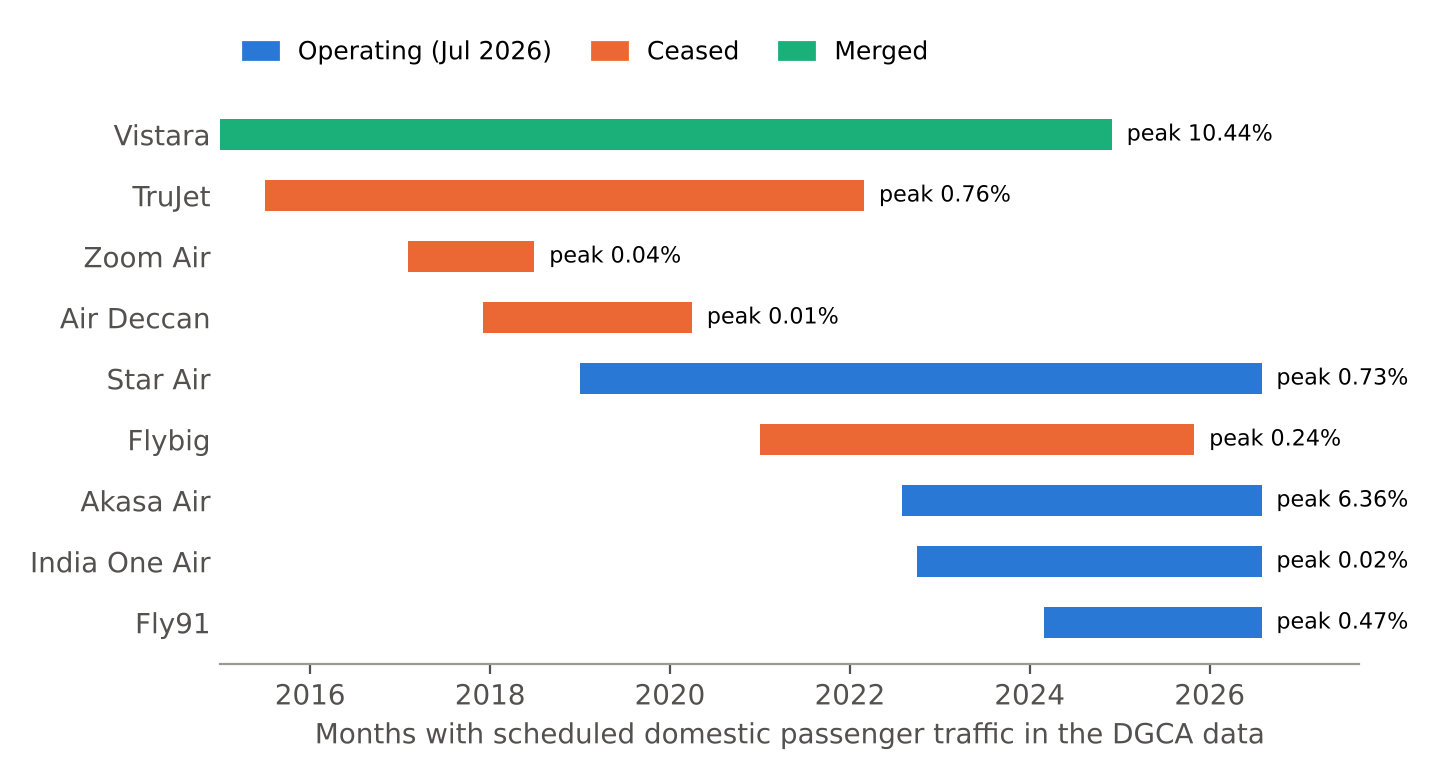
\includegraphics[width=0.92\textwidth]{figures/fig_o3_lifespans.png}
\caption{O3: Operating span and peak passenger share of the nine entrants, January 2015--July 2026; colour shows the outcome at July 2026. Source: DGCA via Kubicek (2026); authors' calculations.}
\label{fig:o3-life}
\end{figure}

\begingroup
\footnotesize
\captionof{table}{O3: All brands first appearing after January 2015 (sensitivity)}
\label{tab:o3-all}
\noindent\begin{tabularx}{\textwidth}{|X|l|l|r|r|l|}
\hline
\textbf{Airline} & \textbf{First} & \textbf{Last} & \textbf{Months} & \textbf{Peak (\%)} & \textbf{Status in this study} \\
\hline
Vistara & Jan 2015 & Nov 2024 & 118 & 10.441 & Team nine \\
\hline
Akasa Air & Aug 2022 & Jul 2026 & 48 & 6.357 & Team nine \\
\hline
TruJet & Jul 2015 & Feb 2022 & 79 & 0.764 & Team nine \\
\hline
Star Air & Jan 2019 & Jul 2026 & 90 & 0.725 & Team nine \\
\hline
Fly91 & Mar 2024 & Jul 2026 & 29 & 0.468 & Team nine \\
\hline
Flybig & Jan 2021 & Oct 2025 & 58 & 0.236 & Team nine \\
\hline
Zoom Air & Feb 2017 & Jun 2018 & 16 & 0.040 & Team nine \\
\hline
India One Air & Oct 2022 & Jul 2026 & 46 & 0.023 & Team nine \\
\hline
Air Deccan & Dec 2017 & Mar 2020 & 13 & 0.012 & Team nine \\
\hline
Air Pegasus & May 2015 & Jul 2016 & 15 & 0.308 & Not in team list \\
\hline
Air Carnival & Aug 2016 & Apr 2017 & 9 & 0.163 & Not in team list \\
\hline
Air Odisha & Feb 2018 & Sep 2018 & 8 & 0.007 & Not in team list \\
\hline
Air Heritage & Jan 2019 & Mar 2020 & 9 & 0.009 & Not in team list \\
\hline
Pawan Hans & May 2019 & Dec 2021 & 29 & 0.004 & Not in team list \\
\hline
Air Taxi & Jan 2021 & Jul 2021 & 7 & 0.004 & Not in team list \\
\hline
AIX Connect & Jan 2024 & Sep 2024 & 9 & 6.115 & Rebrand of AirAsia India \\
\hline
\end{tabularx}
\par\footnotesize Source: DGCA via Kubicek (2026); authors' calculations. AIX Connect is the rebranded AirAsia India, present in the data from January 2015, so it is not an entrant.
\endgroup

\begingroup
\footnotesize
\captionof{table}{O3: Outcome evidence for the nine entrants}
\label{tab:o3-outcomes}
\noindent\begin{tabularx}{\textwidth}{|>{\raggedright\arraybackslash}p{0.13\textwidth}|>{\raggedright\arraybackslash}p{0.12\textwidth}|>{\raggedright\arraybackslash}X|}
\hline
\textbf{Airline} & \textbf{Outcome} & \textbf{Evidence} \\
\hline
Vistara & Merged & Merger completed 12 Nov 2024; Singapore Airlines exchanged its 49\% Vistara stake for 25.1\% of the enlarged Air India (Singapore Airlines, 2025; Tata Sons, 2024). \\
\hline
Akasa Air & Operating & Began flying 7 Aug 2022; 30 aircraft and over 19 million passengers by Aug 2025 (Akasa Air, 2025b). \\
\hline
TruJet & Ceased & Flights suspended 15 Feb 2022 after a cash-flow crisis (ch-aviation, 2022); aircraft repossessed by the lessor (Ministry of Civil Aviation, 2024). A revival was reported as approved in 2025 (Skift, 2025); no traffic after Feb 2022. \\
\hline
Flybig & Ceased & Last traffic Oct 2025; reported to have stopped flying that month, with its operating certificate revoked in Dec 2025 (Allplane, 2025). Check against DGCA records. \\
\hline
Zoom Air & Ceased & Suspended operations in July 2018 (Business Today, 2019); last traffic June 2018 in the data. \\
\hline
Air Deccan & Ceased & Last traffic Mar 2020. The Ministry lists Deccan Charters among airlines that stopped operating after commencement (Ministry of Civil Aviation, 2024); confirm that this is the DGCA's ``Air Deccan''. \\
\hline
Star Air & Operating & Traffic through Jul 2026; listed as operating under UDAN in July 2024 (Ministry of Civil Aviation, 2024). \\
\hline
Fly91 & Operating & Traffic through Jul 2026; listed as operating under UDAN in July 2024 (Ministry of Civil Aviation, 2024). \\
\hline
India One Air & Operating & Traffic through Jul 2026 (46 months); had received its operating certificate by mid-2022 (Business Standard, 2022). \\
\hline
\end{tabularx}
\endgroup




% ===== O3 END =====

\section{Additional Analysis}
Include full regression output, additional calculations, analysis code, or other supporting analysis where applicable.

\textbf{O4 reproduction files.} Data preparation, Python plotting code, numerical tables and run instructions are available in the \href{https://github.com/Goutham7358/Assignment3_Code}{Assignment 3 code repository}.

% ===== O3 START (C) =====
\textbf{O3 reproduction files.} The national entrant tables and figures are produced by \texttt{o3\_entrant\_analysis.py} (submitted with this report), which reads the cleaned DGCA file of Kubicek (2026) at commit \texttt{16770ac}. Route-share and financial calculations are in the \href{https://github.com/Goutham7358/Economics_New_Entrants_India_Domestic_Aviation}{O3 case-study repository}.

% ===== O3 END =====

\section{Survey Questionnaire or Interview Guide}
Include the survey questionnaire or interview guide where applicable.

\newpage
\section*{Methods and Tools Statement}
Provide a short statement covering:
\templatebullet{Data sources used}
\templatebullet{Software or analytical tools used}
\templatebullet{Other relevant tools used in preparing or analysing the study}
\templatebullet{Any AI tool assistance, where applicable}

% ===== O3 START (tools) =====


\textbf{O3 part.} Data: DGCA monthly airline statistics as cleaned by Kubicek (2026); DGCA approved domestic schedules; ICRA rating reports, company releases, regulatory filings and press reports as cited; route and financial inputs and checks are from the team's O3 case-study repository. Tools: Python (pandas, matplotlib) for the entrant calculations and figures, and LaTeX. AI assistance: an AI assistant was used to write the O3 analysis code, draft the O3 text and format it in LaTeX; it was not used to create data or sources, and the O3 author checked the figures against the data and sources and is responsible for the text.


% ===== O3 END =====

\section*{Team Member Contributions}
Provide one line for each team member describing their contribution to the project.

This statement is intended only to confirm that all team members have contributed to the project. It is not an individual assessment of the quality or quantity of each member's contribution, and differences in individual contributions will not result in different marks for team members.
\templatebullet{\textbf{[Member 1]:} [Brief description of contribution.]}
\templatebullet{\textbf{[Member 2]:} [Brief description of contribution.]}
\templatebullet{\textbf{[Member 3]:} [Brief description of contribution.]}
\templatebullet{\textbf{[Member 4]:} [Brief description of contribution.]}

% ===== O3 START (contrib) =====
\templatebullet{\textbf{[O3 member]:} Entrant tracking analysis (national shares, event time, outcomes) and the O3 write-up, using route and financial data prepared by [teammate name].}

% ===== O3 END =====

\newpage
\section*{General Note}
The final report should be around 8--12 pages, excluding references and appendices. There is no strict maximum page limit; the length should be appropriate to the scope and depth of the study.

The sections and subsections may be adapted according to the nature of the research question, data, and methodology. Not every subsection will be applicable to every project.

The final report should maintain a clear connection between the research question, economic framework, data, methodology, analysis, findings, and implications.
\end{document}